\documentclass[aspectratio=169, table]{beamer}

\usepackage{colortbl}
\usepackage{xcolor}
\usepackage{listings}
\usepackage{pgfplots}
\usepgfplotslibrary{polar}
\pgfplotsset{compat=1.18}
\usepackage{tikz}
\usetikzlibrary{shapes.geometric,
	positioning, shapes, shapes.multipart, backgrounds, arrows.meta, calc, fit, trees}

\makeatletter
\def\input@path{{../theme/}}
\makeatother
\graphicspath{{../theme/}}
\usetheme{Pradita}

\lstdefinelanguage{xml}{
	keywords={},
	basicstyle=\ttfamily\scriptsize,
	keywordstyle=\color{blue}\bfseries,
	sensitive=true,
	commentstyle=\color{gray}\ttfamily,
	stringstyle=\color{purple}\ttfamily,
	numbers=left,
	numberstyle=\tiny\color{gray},
	breaklines=true,
	frame=lines,
	backgroundcolor=\color{lightgray!10},
	tabsize=2,
	morecomment=[s]{<!--}{-->},
	morestring=[b]",
	morestring=[b]',
	showstringspaces=false
}

\lstdefinelanguage{java}{
  keywords={package,import,public,class,interface,extends,implements,
            return,new,null,true,false,void,if,else,for,while,static,
            final,private,protected,String,throws,Exception,try,finally,
            boolean,int},
  keywordstyle=\color{blue}\bfseries,
  sensitive=true,
  comment=[l]{//},
  morecomment=[s]{/*}{*/},
  commentstyle=\color{gray}\ttfamily\itshape,
  stringstyle=\color{purple}\ttfamily,
  morestring=[b]",
  basicstyle=\ttfamily\scriptsize,
  numbers=left,
  numberstyle=\tiny\color{gray},
  breaklines=true,
  frame=lines,
  backgroundcolor=\color{lightgray!10},
  showstringspaces=false
}

\lstdefinelanguage{eol}{
  keywords={operation,return,if,else,var,while,for,in,not,and,or,new,self,true,false,null,import,
            context,constraint,critique,check,message,guard,pre,post,Any,String,Boolean,Collection},
  keywordstyle=\color{blue}\bfseries,
  sensitive=true,
  comment=[l]{//},
  morecomment=[s]{/*}{*/},
  commentstyle=\color{gray}\ttfamily\itshape,
  stringstyle=\color{purple}\ttfamily,
  morestring=[b]",
  basicstyle=\ttfamily\scriptsize,
  numbers=left,
  numberstyle=\tiny\color{gray},
  breaklines=true,
  frame=lines,
  backgroundcolor=\color{lightgray!10},
  showstringspaces=false
}

\lstdefinelanguage{mediaflow}{
  keywords={graph,resource,scaler,transcoder,port,edge,from,to,external,true,false,IN,OUT,
            backend,command,replicas,width,height,uri,mediaType},
  keywordstyle=\color{blue}\bfseries,
  sensitive=true,
  comment=[l]{//},
  commentstyle=\color{gray}\ttfamily\itshape,
  stringstyle=\color{purple}\ttfamily,
  morestring=[b]",
  basicstyle=\ttfamily\scriptsize,
  numbers=left,
  numberstyle=\tiny\color{gray},
  breaklines=true,
  frame=lines,
  backgroundcolor=\color{lightgray!10},
  showstringspaces=false
}

\lstdefinelanguage{shell}{
  keywords={cd},
  keywordstyle=\color{blue}\bfseries,
  sensitive=true,
  comment=[l]{\#},
  commentstyle=\color{gray}\ttfamily\itshape,
  stringstyle=\color{purple}\ttfamily,
  basicstyle=\ttfamily\scriptsize,
  numbers=left,
  numberstyle=\tiny\color{gray},
  breaklines=true,
  frame=lines,
  backgroundcolor=\color{lightgray!10},
  showstringspaces=false
}

\lstdefinestyle{ocl}{
  	keywords={package, endpackage, context, inv, def, pre, post, derive, init, body, let, in, if, then, else, endif, and, or, xor, not, implies, true, false, null, invalid, self},
	morekeywords=[2]{Collection, Sequence, Set, OrderedSet, Bag, Map, String, Integer, Real, Boolean, UnlimitedNatural, OclAny, OclVoid, OclInvalid, IN, OUT, VIDEO, AUDIO, IMAGE, FFMPEG, GSTREAMER},
  keywordstyle=\color{blue}\bfseries,
  sensitive=true,
  comment=[l]{//},
  morecomment=[s]{/*}{*/},
  commentstyle=\color{gray}\ttfamily\itshape,
  stringstyle=\color{purple}\ttfamily,
  morestring=[b]",
  basicstyle=\ttfamily\scriptsize,
  numbers=left,
  numberstyle=\tiny\color{gray},
  breaklines=true,
  frame=lines,
  backgroundcolor=\color{lightgray!10},
  showstringspaces=false
}


\subtitle{IT30213 - Advanced Software Engineering \& DevOps}
\title{\Huge Model\vspace{8pt}\\Validation}
\author{\textbf{Alfa Yohannis}}

\begin{document}

\frame{\titlepage}

\begin{frame}[fragile]
	\frametitle{Contents}
	\vspace{20pt}
	\begin{columns}[t]
		\column{0.5\textwidth}
		\tableofcontents[sections={1-4}]

		\column{0.5\textwidth}
		\tableofcontents[sections={5-8}]
	\end{columns}
\end{frame}

\begin{frame}{\hfill}
	\centering
	\Huge{\textbf{Bagaimana memastikan model layak ditransformasikan sebelum M2M dan M2T dijalankan?}}
\end{frame}

% ============================================================
\section{Tujuan Pembelajaran}
\begin{frame}{\hfill}
	\centering
	\Huge{\textbf{Tujuan Pembelajaran}}
\end{frame}

\begin{frame}{Tujuan Pembelajaran}
\vspace{6pt}
Setelah sesi ini, mahasiswa diharapkan mampu:
\begin{enumerate}
  \item Menjelaskan peran validasi model dalam siklus \textit{Model-Driven Engineering} sebagai gerbang kualitas sebelum M2M dan M2T.
  \item Menerapkan validasi model \textit{MediaFlow} menggunakan EVL dan OCL, termasuk helper, constraint, guard, message, dan critique.
  \item Menganalisis trade-off EVL dan OCL dari sisi ekspresivitas, keterbacaan, pelaporan error, formalitas, dan integrasi Java.
\end{enumerate}
\end{frame}

% ============================================================
\section{Pendahuluan}
\begin{frame}{\hfill}
	\centering
	\Huge{\textbf{Pendahuluan}}
\end{frame}

\begin{frame}{Mengapa Metamodel Saja Tidak Cukup?}
\vspace{6pt}
\begin{columns}[T]
\column{0.5\textwidth}
\textbf{Yang dapat dijamin Ecore}
\begin{itemize}
  \item Tipe atribut dan referensi.
  \item Kardinalitas containment.
  \item Struktur dasar \texttt{Graph}, \texttt{Node}, \texttt{Edge}, \texttt{Port}.
\end{itemize}

\column{0.5\textwidth}
\textbf{Yang tidak dijamin Ecore}
\begin{itemize}
  \item Edge mengalir \texttt{OUT $\rightarrow$ IN}.
  \item Nama node unik sebagai identifier.
  \item URI resource memakai scheme yang dikenal.
  \item Bitrate dan resolusi masuk akal.
\end{itemize}
\end{columns}

\vspace{8pt}
\textbf{Konsekuensi:} tanpa validasi, M2M dan M2T dapat menerima model yang tampak sah secara struktur tetapi salah secara semantik domain.
\end{frame}

\begin{frame}{Posisi Validasi dalam MDE}
\vspace{6pt}
\centering
\scalebox{0.85}{
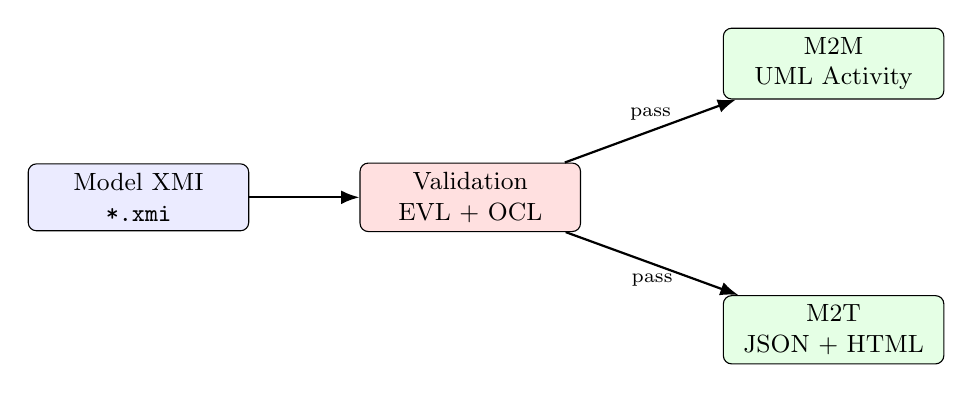
\begin{tikzpicture}[>=Latex, node distance=12mm,
  box/.style={draw, rounded corners=3pt, minimum width=2.8cm, minimum height=0.85cm, align=center, fill=blue!8, font=\small},
  gate/.style={draw, rounded corners=3pt, minimum width=2.8cm, minimum height=0.85cm, align=center, fill=red!12, font=\small},
  target/.style={draw, rounded corners=3pt, minimum width=2.8cm, minimum height=0.85cm, align=center, fill=green!10, font=\small}]
  \node[box] (model) {Model XMI\\\texttt{*.xmi}};
  \node[gate, right=14mm of model] (val) {Validation\\EVL + OCL};
  \node[target, above right=8mm and 18mm of val] (m2m) {M2M\\UML Activity};
  \node[target, below right=8mm and 18mm of val] (m2t) {M2T\\JSON + HTML};

  \draw[->, thick] (model) -- (val);
  \draw[->, thick] (val) -- node[above, font=\scriptsize] {pass} (m2m);
  \draw[->, thick] (val) -- node[below, font=\scriptsize] {pass} (m2t);
\end{tikzpicture}
}

\vspace{8pt}
\small
Validasi adalah \textit{quality gate}: model invalid berhenti lebih awal dengan diagnostik yang konkret.
\end{frame}

% ============================================================
\section{Masalah Domain}
\begin{frame}{\hfill}
	\centering
	\Huge{\textbf{Masalah Domain}}
\end{frame}

\begin{frame}{Korpus Validasi}
\vspace{2pt}
\scriptsize
\begin{tabular}{|p{0.26\textwidth}|p{0.16\textwidth}|p{0.50\textwidth}|}
\hline
\rowcolor{black!8}
\textbf{Model Input} & \textbf{Kategori} & \textbf{Tujuan Pengujian} \\
\hline
\texttt{linear-resize.xmi} & Valid & Pipeline linier: input, satu scaler, output. \\
\hline
\texttt{adaptive-delivery.xmi} & Valid & Pipeline bercabang: hasil resize ke dua format. \\
\hline
\texttt{broken-direction.xmi} & Invalid & Arah edge salah, command kosong, replika nol, dimensi 0, URI kosong. \\
\hline
\texttt{duplicate-and-isolated.xmi} & Invalid & Duplikasi nama, port tak terpakai, self-loop, scheme URI, codec/container, warning replika. \\
\hline
\end{tabular}

\vspace{8pt}
\small
Dua model valid menjaga validator tidak terlalu ketat; dua model invalid memastikan tiap aturan benar-benar mendeteksi pelanggaran.
\end{frame}

\begin{frame}{Kategori Aturan Validasi}
\vspace{2pt}
\scriptsize
\begin{tabular}{|p{0.20\textwidth}|p{0.72\textwidth}|}
\hline
\rowcolor{black!8}
\textbf{Konteks} & \textbf{Aturan Utama} \\
\hline
\texttt{Graph} & Nama wajib, tidak kosong, nama node/edge unik, ada entry dan exit eksternal, tidak ada node terisolasi. \\
\hline
\texttt{Node} & Wajib bernama, memiliki port, port unik dalam satu node. \\
\hline
\texttt{Port} & Wajib bernama, berpartisipasi minimal pada satu edge. \\
\hline
\texttt{Edge} & Wajib bernama, source dan target ada, \texttt{OUT $\rightarrow$ IN}, bukan self-loop. \\
\hline
\texttt{Resource} & URI ada, scheme dikenal, eksternal hanya input atau output saja. \\
\hline
\texttt{Transformer} & Command ada, replika $\geq$ 1, ada incoming dan outgoing, warning replika besar. \\
\hline
\texttt{Scaler} & Width dan height positif, tidak melebihi 8K. \\
\hline
\texttt{Transcoder} & Codec/container ada, bitrate masuk akal, kombinasi container-codec plausibel. \\
\hline
\end{tabular}
\end{frame}

\begin{frame}[fragile]{Contoh Model Invalid: Broken Direction}
\vspace{2pt}
\begin{columns}[T,onlytextwidth]
\column{0.66\textwidth}
\begin{lstlisting}[language=mediaflow, basicstyle=\ttfamily\tiny]
graph brokenDirection {
  resource inputVideo [mediaType=VIDEO]
    uri="file:///home/alfa/videos/input.mp4"
    external=true {
    port inputOut OUT
  }

  scaler resize720 backend=FFMPEG command=""
    replicas=0 width=0 height=720 {
    port resizeIn IN
    port resizeOut OUT
  }

  resource outputVideo [mediaType=VIDEO] uri=""
    external=true {
    port outputIn IN
  }

  edge e1 from inputOut to resizeIn
  edge e2 from outputIn to resizeOut
}
\end{lstlisting}

\column{0.31\textwidth}
\scriptsize
\textbf{Pelanggaran sengaja}
\begin{itemize}
  \item \texttt{e2} arahnya \texttt{IN $\rightarrow$ OUT}.
  \item Command scaler kosong.
  \item Replika nol, width nol.
  \item URI output kosong.
  \item Satu model kecil, banyak constraint.
\end{itemize}
\end{columns}
\end{frame}

\begin{frame}{Visualisasi Pelanggaran Edge \texttt{e2}}
\vspace{4pt}
\centering
\scalebox{1}{
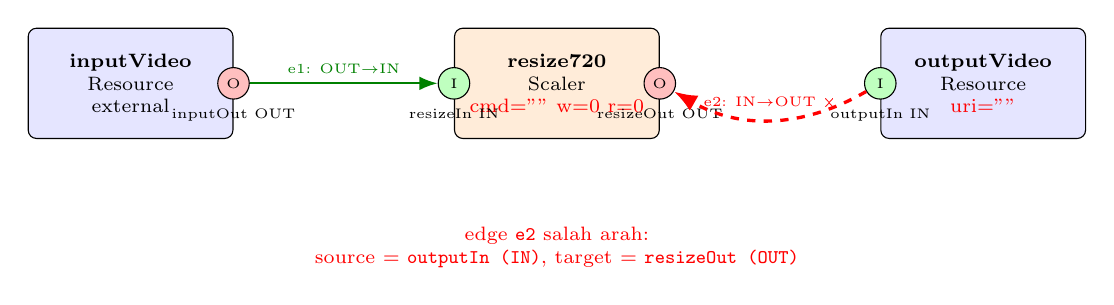
\begin{tikzpicture}[>=Latex,
  node/.style={draw, rounded corners=3pt, minimum width=2.6cm, minimum height=1.4cm, align=center, font=\scriptsize},
  res/.style={node, fill=blue!10},
  scl/.style={node, fill=orange!15},
  port/.style={draw, circle, inner sep=0pt, minimum size=4mm, font=\tiny, fill=white},
  portIn/.style={port, fill=green!25},
  portOut/.style={port, fill=red!25},
  ok/.style={->, thick, green!50!black},
  bad/.style={->, very thick, red, dashed}]

  \node[res] (in) {\textbf{inputVideo}\\Resource\\external};
  \node[scl, right=28mm of in] (sc) {\textbf{resize720}\\Scaler\\\textcolor{red}{cmd="" w=0 r=0}};
  \node[res, right=28mm of sc] (out) {\textbf{outputVideo}\\Resource\\\textcolor{red}{uri=""}};

  \node[portOut] (inOut) at ($(in.east)+(0,0)$) {\tiny O};
  \node[portIn]  (scIn)  at ($(sc.west)+(0,0)$) {\tiny I};
  \node[portOut] (scOut) at ($(sc.east)+(0,0)$) {\tiny O};
  \node[portIn]  (outIn) at ($(out.west)+(0,0)$) {\tiny I};

  \node[font=\tiny, below=0pt of inOut] {inputOut OUT};
  \node[font=\tiny, below=0pt of scIn]  {resizeIn IN};
  \node[font=\tiny, below=0pt of scOut] {resizeOut OUT};
  \node[font=\tiny, below=0pt of outIn] {outputIn IN};

  \draw[ok] (inOut) -- node[above, font=\tiny, green!50!black] {e1: OUT$\rightarrow$IN \checkmark} (scIn);
  \draw[bad] (outIn) to[bend left=30] node[above, font=\tiny, red] {e2: IN$\rightarrow$OUT \texttimes} (scOut);

  \node[font=\scriptsize, red, below=10mm of sc, align=center] (label) {edge \texttt{e2} salah arah:\\source = \texttt{outputIn (IN)}, target = \texttt{resizeOut (OUT)}};
\end{tikzpicture}
}

\vspace{6pt}
\small
Hijau: edge sah (\texttt{OUT$\rightarrow$IN}). Merah putus-putus: edge \texttt{e2} melanggar \texttt{ConnectsOutputToInput}; akibatnya resource output tidak lagi menjadi exit boundary, memicu \texttt{HasExternalEntryAndExit}.
\end{frame}

% ============================================================
\section{Arsitektur Validasi}
\begin{frame}{\hfill}
	\centering
	\Huge{\textbf{Arsitektur Validasi}}
\end{frame}

\begin{frame}{Pipeline Proyek \texttt{model-validation}}
\vspace{4pt}
\centering
\scalebox{.9}{
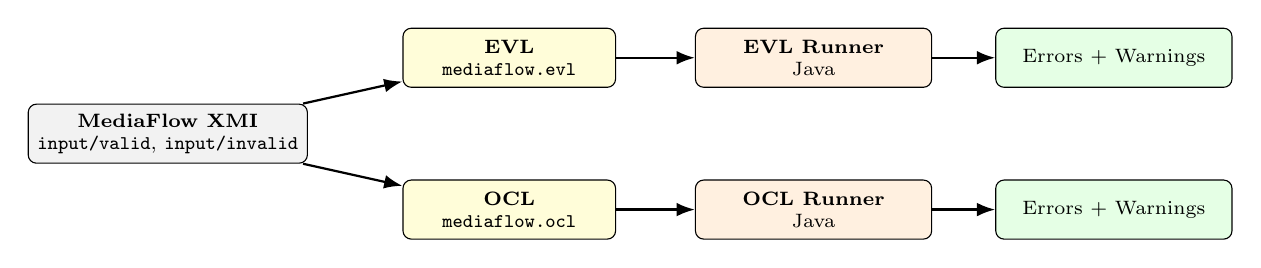
\begin{tikzpicture}[>=Latex,
  box/.style={draw, rounded corners=3pt, minimum width=2.7cm, minimum height=0.75cm, align=center, font=\scriptsize},
  spec/.style={draw, rounded corners=3pt, minimum width=2.7cm, minimum height=0.75cm, align=center, font=\scriptsize, fill=yellow!15},
  runner/.style={draw, rounded corners=3pt, minimum width=3.0cm, minimum height=0.75cm, align=center, font=\scriptsize, fill=orange!12},
  outbox/.style={draw, rounded corners=3pt, minimum width=3.0cm, minimum height=0.75cm, align=center, font=\scriptsize, fill=green!10}]

  \node[box, fill=gray!10] (xmi) {\textbf{MediaFlow XMI}\\\texttt{input/valid}, \texttt{input/invalid}};

  \node[spec, above right=2mm and 12mm of xmi] (evl) {\textbf{EVL}\\\texttt{mediaflow.evl}};
  \node[spec, below right=2mm and 12mm of xmi] (ocl) {\textbf{OCL}\\\texttt{mediaflow.ocl}};

  \node[runner, right=10mm of evl] (rEvl) {\textbf{EVL Runner}\\Java};
  \node[runner, right=10mm of ocl] (rOcl) {\textbf{OCL Runner}\\Java};

  \node[outbox, right=8mm of rEvl] (oEvl) {Errors + Warnings};
  \node[outbox, right=8mm of rOcl] (oOcl) {Errors + Warnings};

  \draw[->, thick] (xmi) -- (evl);
  \draw[->, thick] (xmi) -- (ocl);
  \draw[->, thick] (evl) -- (rEvl);
  \draw[->, thick] (ocl) -- (rOcl);
  \draw[->, thick] (rEvl) -- (oEvl);
  \draw[->, thick] (rOcl) -- (oOcl);
\end{tikzpicture}
}
\vspace{6pt}
\small
EVL adalah validator utama; OCL menjadi spesifikasi formal pendamping atas metamodel yang sama.
\end{frame}

\begin{frame}[fragile]{Struktur Proyek}
\vspace{2pt}
\begin{columns}[T,onlytextwidth]
\column{0.66\textwidth}
\begin{lstlisting}[basicstyle=\ttfamily\tiny, breaklines=true]
model-validation/
|-- src/validation/
|   |-- MediaflowEvlValidationRunner.java
|   +-- MediaflowOclValidationRunner.java
|-- validator/
|   |-- mediaflow.evl
|   +-- mediaflow.ocl
|-- input/
|   |-- valid/
|   |   |-- linear-resize.xmi
|   |   +-- adaptive-delivery.xmi
|   +-- invalid/
|       |-- broken-direction.xmi
|       +-- duplicate-and-isolated.xmi
|-- run-evl-validation.sh
|-- run-ocl-validation.sh
+-- pom.xml
\end{lstlisting}

\column{0.31\textwidth}
\scriptsize
\textbf{Penjelasan singkat}
\begin{itemize}
  \item \texttt{src/}: dua runner Java.
  \item \texttt{validator/}: EVL dan OCL.
  \item \texttt{input/}: korpus valid dan invalid.
  \item Metamodel dirujuk dari proyek \texttt{mediaflow}.
\end{itemize}
\end{columns}
\end{frame}

\begin{frame}{Metodologi 7 Langkah}
\vspace{6pt}
\begin{enumerate}\small
  \item Mengidentifikasi \textit{invariant} dari M2M dan M2T sebelumnya.
  \item Menyusun korpus valid dan invalid.
  \item Mendefinisikan helper navigasi (port-ke-node, node-ke-edge).
  \item Menulis constraint EVL dengan message dan guard.
  \item Menulis spesifikasi OCL pendamping.
  \item Mengimplementasikan runner Java untuk EVL dan OCL.
  \item Mengevaluasi hasil pada seluruh korpus.
\end{enumerate}
\end{frame}

% ============================================================
\section{Implementasi EVL}
\begin{frame}{\hfill}
	\centering
	\Huge{\textbf{Implementasi EVL}}
\end{frame}

\begin{frame}[fragile]{Helper EVL: Navigasi Model}
\vspace{2pt}
\begin{columns}[T,onlytextwidth]
\column{0.66\textwidth}
\begin{lstlisting}[language=eol, basicstyle=\ttfamily\tiny]
operation Any hasText() : Boolean {
    return self.isDefined() and self.asString().trim().length() > 0;
}

operation Mediaflow!Port isOut() : Boolean {
    return self.direction.toString() == "OUT";
}

operation Mediaflow!Port ownerNode() : Any {
    return Mediaflow!Node.all.selectOne(node |
        node.ports.includes(self));
}

operation Mediaflow!Node incomingEdges() : Collection {
    return Mediaflow!Edge.all.select(edge |
        edge.target.isDefined() and self.ports.includes(edge.target));
}
\end{lstlisting}

\column{0.31\textwidth}
\scriptsize
\textbf{Penjelasan singkat}
\begin{itemize}
  \item \texttt{hasText()} cek string non-kosong.
  \item \texttt{isOut()} arah port.
  \item \texttt{ownerNode()} resolusi port-ke-node.
  \item \texttt{incomingEdges()} menyusun edge masuk.
  \item Helper dipakai ulang oleh banyak constraint.
\end{itemize}
\end{columns}
\end{frame}

\begin{frame}[fragile]{Constraint: Graph, Node, Port}
\vspace{2pt}
\begin{columns}[T,onlytextwidth]
\column{0.66\textwidth}
\begin{lstlisting}[language=eol, basicstyle=\ttfamily\tiny]
context Mediaflow!Graph {
    constraint HasName {
        check : self.name.hasText()
        message : "Graph must have a non-empty name."
    }
    constraint UniqueNodeNames {
        check : self.nodes.haveUniqueNames()
        message : "Graph '" + self.label() +
            "' has duplicate or missing node names."
    }
}

context Mediaflow!Port {
    constraint PortParticipatesInAnEdge {
        check : not self.incidentEdges().isEmpty()
        message : "Port '" + self.label() +
            "' is not used by any edge."
    }
}
\end{lstlisting}

\column{0.31\textwidth}
\scriptsize
\textbf{Penjelasan singkat}
\begin{itemize}
  \item Constraint dekat dengan elemen yang divalidasi.
  \item Pesan menyebut nama elemen.
  \item Aturan terkait M2T: nama unik untuk identifier output.
\end{itemize}
\end{columns}
\end{frame}

\begin{frame}[fragile]{Constraint: Edge dengan Guard}
\vspace{2pt}
\begin{columns}[T,onlytextwidth]
\column{0.66\textwidth}
\begin{lstlisting}[language=eol, basicstyle=\ttfamily\tiny]
context Mediaflow!Edge {

    constraint EndpointsAreDeclared {
        check : self.source.isDefined() and self.target.isDefined()
        message : "Edge '" + self.label() +
            "' must declare both source and target ports."
    }

    constraint ConnectsOutputToInput {
        guard : self.source.isDefined() and self.target.isDefined()
        check : self.source.isOut() and self.target.isIn()
        message : "Edge '" + self.label() +
            "' must connect an OUT port to an IN port."
    }

    constraint ConnectsDifferentNodes {
        guard : self.source.isDefined() and self.target.isDefined()
        check : not (self.sourceNode() == self.targetNode())
        message : "Edge '" + self.label() +
            "' connects two ports on the same node."
    }
}
\end{lstlisting}

\column{0.31\textwidth}
\scriptsize
\textbf{Penjelasan singkat}
\begin{itemize}
  \item \texttt{guard} mencegah error berantai.
  \item Tanpa guard, akses \texttt{source.direction} bisa gagal teknis.
  \item Pesan tetap fokus pada akar masalah.
\end{itemize}
\end{columns}
\end{frame}

\begin{frame}[fragile]{Critique: Warning untuk Worker Berlebih}
\vspace{2pt}
\begin{columns}[T,onlytextwidth]
\column{0.66\textwidth}
\begin{lstlisting}[language=eol, basicstyle=\ttfamily\tiny]
context Mediaflow!Transformer {

    constraint ReplicasArePositive {
        check : self.replicas >= 1
        message : "Transformer '" + self.label() +
            "' must request at least one replica."
    }

    critique TooManyWorkers {
        check : self.replicas <= 4
        message : "Transformer '" + self.label() +
            "' requests " + self.replicas +
            " worker replicas. Use 4 or fewer."
    }
}

context Mediaflow!Scaler {
    constraint DimensionsArePositive {
        check : self.width > 0 and self.height > 0
        message : "Scaler '" + self.label() +
            "' must have positive width and height."
    }
}
\end{lstlisting}

\column{0.31\textwidth}
\scriptsize
\textbf{Penjelasan singkat}
\begin{itemize}
  \item \texttt{constraint}: error keras.
  \item \texttt{critique}: warning, bukan blocker.
  \item Tidak semua kualitas adalah pelanggaran fatal.
  \item OCL standar tidak punya \texttt{critique}.
\end{itemize}
\end{columns}
\end{frame}

% ============================================================
\section{Implementasi OCL dan Runner}
\begin{frame}{\hfill}
	\centering
	\Huge{\textbf{Implementasi OCL dan Runner}}
\end{frame}

\begin{frame}[fragile]{Spesifikasi OCL Pendamping}
\vspace{2pt}
\begin{columns}[T,onlytextwidth]
\column{0.66\textwidth}
\begin{lstlisting}[style=ocl, basicstyle=\ttfamily\tiny]
package mediaflow

context Graph
inv UniqueNodeNames:
    self.nodes->isUnique(name)

context Edge
inv ConnectsOutputToInput:
    self.source <> null and self.target <> null implies
    (self.source.direction = Direction::OUT and
     self.target.direction = Direction::IN)

context Transformer
inv ReplicasArePositive:
    self.replicas >= 1

context Scaler
inv DimensionsArePositive:
    self.width > 0 and self.height > 0

context Transcoder
inv BitrateIsPlausible:
    self.bitrate >= 128 and self.bitrate <= 50000

endpackage
\end{lstlisting}

\column{0.31\textwidth}
\scriptsize
\textbf{Penjelasan singkat}
\begin{itemize}
  \item OCL ringkas untuk invariant murni.
  \item Tidak menyimpan pesan per constraint.
  \item Runner mencetak nama dan ekspresi yang gagal.
  \item Cocok sebagai kontrak deklaratif.
\end{itemize}
\end{columns}
\end{frame}

\begin{frame}[fragile]{Runner EVL: Alur Utama}
\vspace{2pt}
\begin{columns}[T,onlytextwidth]
\column{0.66\textwidth}
\begin{lstlisting}[language=java, basicstyle=\ttfamily\tiny]
String inputPath = args.length > 0 ? args[0] : "input";
String evlPath = args.length > 1 ? args[1] :
    "validator/mediaflow.evl";
String metamodelPath = args.length > 2 ? args[2] :
    "../mediaflow/metamodels/mediaflow.ecore";

registerFactories();

List<Path> inputs = collectInputs(Paths.get(inputPath));
int errorCount = 0;
int warningCount = 0;

for (Path input : inputs) {
    ValidationSummary summary = validate(input,
        Paths.get(evlPath), Paths.get(metamodelPath));
    errorCount += summary.errors;
    warningCount += summary.warnings;
}

if (errorCount > 0) { System.exit(1); }
\end{lstlisting}

\column{0.31\textwidth}
\scriptsize
\textbf{Penjelasan singkat}
\begin{itemize}
  \item Argumen CLI fleksibel.
  \item \texttt{collectInputs()} rekursif untuk \texttt{*.xmi}.
  \item Akumulasi error dan warning.
  \item Exit code 1 jika ada error: ramah CI.
\end{itemize}
\end{columns}
\end{frame}

\begin{frame}[fragile]{Pelaporan Hasil EVL}
\vspace{2pt}
\begin{columns}[T,onlytextwidth]
\column{0.66\textwidth}
\begin{lstlisting}[language=java, basicstyle=\ttfamily\tiny]
for (UnsatisfiedConstraint result : unsatisfied) {
    boolean warning = result.getConstraint().isCritique();
    if (warning) {
        warnings++;
    } else {
        errors++;
    }

    String severity = warning ? "WARN" : "ERROR";
    String counter = warning ? "W" + warnings
                             : String.valueOf(errors);
    System.out.println(counter + ". " + severity + " " +
        result.getConstraint().getName() + " on " +
        describe(result.getInstance()) + ": " +
        result.getMessage());
}
\end{lstlisting}

\column{0.31\textwidth}
\scriptsize
\textbf{Penjelasan singkat}
\begin{itemize}
  \item \texttt{isCritique()} membedakan severity.
  \item \texttt{describe()} memakai nama \texttt{EObject}.
  \item Output mudah ditelusuri ke model sumber.
\end{itemize}
\end{columns}
\end{frame}

\begin{frame}[fragile]{Runner OCL: Eksekusi Invariant}
\vspace{2pt}
\begin{columns}[T,onlytextwidth]
\column{0.66\textwidth}
\begin{lstlisting}[language=java, basicstyle=\ttfamily\tiny]
List<OclInvariant> invariants = parseInvariants(Paths.get(oclPath));

ResourceSet resourceSet = new ResourceSetImpl();
EPackage mediaflowPackage = loadMetamodel(resourceSet, metamodelPath);
Resource model = resourceSet.getResource(
    URI.createFileURI(input.toAbsolutePath().toString()), true);

Map<EClass, Set<EObject>> extentMap =
    buildExtentMap(mediaflowPackage, model);

OCL ocl = OCL.newInstance(
    new EcoreEnvironmentFactory(resourceSet.getPackageRegistry()));
ocl.setExtentMap(extentMap);

for (OclInvariant inv : invariants) {
    EClass context = findContext(mediaflowPackage, inv.contextName);
    Constraint c = compileInvariant(ocl, context, inv);
    for (EObject instance : extentMap.getOrDefault(context, Set.of())) {
        if (!ocl.check(instance, c)) { /* report */ }
    }
}
\end{lstlisting}

\column{0.31\textwidth}
\scriptsize
\textbf{Penjelasan singkat}
\begin{itemize}
  \item Parse Complete OCL berbasis teks.
  \item \texttt{extentMap} untuk \texttt{allInstances()}.
  \item Setiap instance di-cek satu per satu.
  \item Warning dipetakan dari daftar invariant tertentu.
\end{itemize}
\end{columns}
\end{frame}

\begin{frame}[fragile]{Skrip Eksekusi}
\vspace{2pt}
\begin{lstlisting}[language=shell, basicstyle=\ttfamily\scriptsize]
cd projects/session-13/model-validation

./run-evl-validation.sh input/valid
./run-evl-validation.sh input/invalid

./run-ocl-validation.sh input/valid
./run-ocl-validation.sh input/invalid
\end{lstlisting}

\vspace{6pt}
\small
Argumen CLI sejajar antar runner:
\begin{itemize}\scriptsize
  \item \texttt{MediaflowEvlValidationRunner [input] [evlPath] [metamodelPath]}
  \item \texttt{MediaflowOclValidationRunner [input] [oclPath] [metamodelPath]}
\end{itemize}
Default: \texttt{input/}, \texttt{validator/}, dan \texttt{../mediaflow/metamodels/mediaflow.ecore}.
\end{frame}

% ============================================================
\section{Evaluasi}
\begin{frame}{\hfill}
	\centering
	\Huge{\textbf{Evaluasi}}
\end{frame}

\begin{frame}{Hasil pada Seluruh Korpus}
\vspace{6pt}
\centering
\scriptsize
\begin{tabular}{|p{0.30\textwidth}|c|c|p{0.40\textwidth}|}
\hline
\rowcolor{black!8}
\textbf{Model Input} & \textbf{Error} & \textbf{Warn} & \textbf{Catatan} \\
\hline
\texttt{linear-resize.xmi} & 0 & 0 & Pipeline linier valid. \\
\hline
\texttt{adaptive-delivery.xmi} & 0 & 0 & Pipeline bercabang valid. \\
\hline
\texttt{broken-direction.xmi} & 8 & 0 & Arah edge, URI, command, replika, dimensi. \\
\hline
\texttt{duplicate-and-isolated.xmi} & 9 & 1 & Duplikasi, port yatim, self-loop, codec; warning replika. \\
\hline
\textbf{Total} & \textbf{17} & \textbf{1} & EVL dan OCL menghasilkan jumlah sama. \\
\hline
\end{tabular}

\vspace{8pt}
\small
Dua model valid lolos tanpa false positive; dua model invalid memicu seluruh kategori constraint.
\end{frame}

\begin{frame}[fragile]{Contoh Output EVL}
\vspace{2pt}
\begin{lstlisting}[language=shell, basicstyle=\ttfamily\tiny]
== input/invalid/broken-direction.xmi ==
1. ERROR HasExternalEntryAndExit on Graph 'brokenDirection':
   Graph 'brokenDirection' must have at least one external entry resource and one external exit resource.
2. ERROR ConnectsOutputToInput on Edge 'e2':
   Edge 'e2' must connect an OUT port to an IN port.
3. ERROR UriIsDeclared on Resource 'outputVideo':
   Resource 'outputVideo' must declare a URI.
4. ERROR CommandIsDeclared on Scaler 'resize720':
   Transformer 'resize720' must declare the command it will execute.
5. ERROR ReplicasArePositive on Scaler 'resize720':
   Transformer 'resize720' must request at least one replica.
6. ERROR DimensionsArePositive on Scaler 'resize720':
   Scaler 'resize720' must have positive width and height.
Displayed 8 error(s), 0 warning(s), 8 total issue(s).
\end{lstlisting}

\vspace{4pt}
\small
Setiap baris menyebut severity, nama constraint, target instance, dan pesan kontekstual.
\end{frame}

\begin{frame}{Perbandingan EVL vs OCL: Aspek Teknis}
\vspace{2pt}
\scriptsize
\begin{tabular}{|p{0.18\textwidth}|p{0.36\textwidth}|p{0.36\textwidth}|}
\hline
\rowcolor{black!8}
\textbf{Aspek} & \textbf{EVL} & \textbf{OCL} \\
\hline
Tujuan & Validasi eksekutabel dengan pesan ramah pengguna. & Spesifikasi invariant formal. \\
\hline
Struktur & \texttt{constraint}, \texttt{check}, \texttt{message}, \texttt{guard}, \texttt{critique}. & \texttt{inv} dan ekspresi Boolean. \\
\hline
Pesan & Melekat pada constraint via \texttt{message}. & Tidak melekat; runner yang mengatur. \\
\hline
Warning & \texttt{critique} bawaan. & Tidak ada; perlu mapping di runner. \\
\hline
Helper & Operation EOL fleksibel. & Lebih terbatas pada setup ini. \\
\hline
Integrasi & \texttt{EvlModule} mengembalikan \texttt{UnsatisfiedConstraint}. & Compile dan check per instance. \\
\hline
Pembelajaran & Validasi end-to-end. & Kontrak metamodel formal. \\
\hline
\end{tabular}
\end{frame}

\begin{frame}{Panduan Pemilihan}
\vspace{6pt}
\begin{itemize}
  \item \textbf{Pilih EVL} ketika validator dipakai langsung pemodel atau pipeline otomatis. Lebih kuat pada pesan diagnostik, severity, guard, dan helper eksekutabel.
  \item \textbf{Pilih OCL} ketika aturan didokumentasikan sebagai invariant formal yang ringkas, dekat dengan standar pemodelan.
  \item \textbf{Gunakan keduanya} untuk pembelajaran atau verifikasi silang: EVL sebagai eksekusi utama, OCL sebagai kontrak deklaratif.
\end{itemize}
\end{frame}

% ============================================================
\section{Pitfall dan Ringkasan}
\begin{frame}{\hfill}
	\centering
	\Huge{\textbf{Pitfall dan Ringkasan}}
\end{frame}

\begin{frame}{Pitfall Umum Validasi Model}
\vspace{6pt}
\begin{itemize}\small
  \item \textbf{Mengandalkan metamodel saja:} Ecore tidak menjamin aturan domain seperti \texttt{OUT $\rightarrow$ IN}.
  \item \textbf{Constraint berantai:} satu kesalahan memicu banyak error; pesan harus jelas.
  \item \textbf{Lupa guard:} akses \texttt{source.direction} tanpa cek dapat gagal teknis.
  \item \textbf{Duplikasi nama dianggap sepele:} M2T memakai nama untuk file/id; duplikasi merusak output.
  \item \textbf{Port tak terpakai:} valid struktur, tetapi membingungkan transformasi.
  \item \textbf{OCL \texttt{allInstances()}:} butuh \texttt{extentMap} pada eksekusi programatik.
  \item \textbf{Warning sebagai error:} hilangkan dengan \texttt{critique}.
  \item \textbf{Classpath Eclipse:} EMF, Epsilon, OCL, LPG, Guava, Apache Commons harus lengkap.
\end{itemize}
\end{frame}

\begin{frame}{Ringkasan}
\vspace{6pt}
\begin{itemize}
  \item Validasi model adalah lapisan penting MDE setelah modeling, M2M, dan M2T.
  \item Pada \textit{MediaFlow}, validasi menjaga precondition: entry/exit, arah edge, nama unik, URI, command, dan parameter media.
  \item Proyek \texttt{model-validation} menerapkan EVL (pragmatis, eksekutabel) dan OCL (formal, deklaratif).
  \item Kedua runner Java menghasilkan evaluasi konsisten: 17 error dan 1 warning pada korpus sesi 13.
  \item Validasi sebelum transformasi membuat pipeline MDE lebih aman: model yang salah berhenti lebih awal dengan diagnostik konkret.
\end{itemize}
\end{frame}

\end{document}
